\section{Perception}
\label{sec:perception}

The three perception components are
shown in \cref{fig:software_overview}.
\begin{itemize}
    \item \textbf{Object detection and classification:}
      Generates 2D object proposals and classifies them in a
      binary way based on a provided target class, resulting
      in the proposals being classified as either target
      class or not. 
      Object detection and classification are realized using
      two different models. Both models are fine-tuned on a 
      supermarket dataset, but do not require retraining to
      add new products, as we will explain in the following.
    \item \textbf{Object pose estimation:} Uses 2D object
      proposals in combination with a depth image to convert
      them to 3D. To estimate the orientation around the
      z-axis, we use a plane-fit of the pointcloud frustum.
      That first order approximation of the surface of the
      products front has proven to be a reliable approach,
      even for non-planar surfaces, see
      \cref{fig:product_examples}.
    \item \textbf{Multi-object tracking:} To track the
      objects over time, we use a set of Kalman Filters, one
      per object. The object proposals are assigned to
      Kalman Filter tracks using the Hungarian Algorithm
      \cite{hamuda2018improved,sahbani2016kalman}.
\end{itemize}

Because a supermarket has a large and often changing set of
products, the main requirement for our perception pipeline
is that it should be easily adaptable. This observation from
retail environments led us to the constraint on the
perception pipeline that it should not require retraining
when new products are added. Such a constraint can be
addressed using, so-called, \textit{few-shot} models.
In the
following, we describe the details of our object detection
and classification method.

The method utilizes YOLO for object detection, relying on
product details for object classification. Additionally, our
system allows adding products using a
single or few images.

This dynamic addition of new products is possible trough a
few-shot model we dub ProtoProductNet. This model is based
on ProtoNet \cite{protonet_2017}. ProtoNet matches query
images to target classes by their distance in feature space.
For each target class a prototype is constructed that is
essentially the mean of the features of a number of example
images of this class. By matching query images to target
prototypes, ProtoNet essentially learns to encode features
that classify similarity between query images and target
classes. Because this model picks random query- and target
classes from a dataset for every iteration, ProtoNet learns
a general feature extraction strategy that is invariant of the
actual class. This is important for adding new
products, as classifying new products is as easy as
providing the model with new target images.

The exact implementation of ProtoNet we use is based on P$>$M$>$F \cite{pmf_2022}. P$>$M$>$F shows that in few-shot learning pre-training (P) is more important than meta-training (M), which is in turn more important than fine-tuning (F). For the best results the authors of P$>$M$>$F suggest using ProtoNet with a Vision Transformer pre-trained with DINO \cite{dino_2021} as the feature extractor and meta-training it with a small learning rate.

However like most few-shot classification models, ProtoNet assumes that query images can only be one  target class. Not only would comparing a query image to all supermarket products increase inference time, attributing it to a likeliest product is unsafe. If our product detector misidentifies a human as a product, the classifier must correctly recognize that and not classify it as the most likely product.

ProtoProductNet makes exactly this possible. It uses a ViT pre-trained with DINO to extract image features, and predicts if those features are part of a target prototype based on their cosine distance. ProtoProductNet then passes this cosine distance through a linear layer combined with a sigmoid function to translate it to a confidence score. If query images have a confidence $<0.5$, they are considered not the target class. Using a sigmoid function however leads to a loss of relational information between classes. In contrast to ProtoNet, that predicts only the most likely target class among a set of target classes with a softmax function, a sigmoid predictor only uses the cosine distance per class to make predictions. As this mechanic is an important reason why ProtoNet works so well, ProtoProductNet will also be allowed to choose the likeliest from a number of prototypes. This means that next to a target prototype, a number of helper prototypes will be chosen. When classes are likelier to be a helper class then the target class, they are considered to be not the target class. As classes that are close together in feature space are harder to distinguish, it makes only sense to choose helper prototypes that are close to the target prototype.

% \begin{figure}[ht]
  % \begin{center}
    % 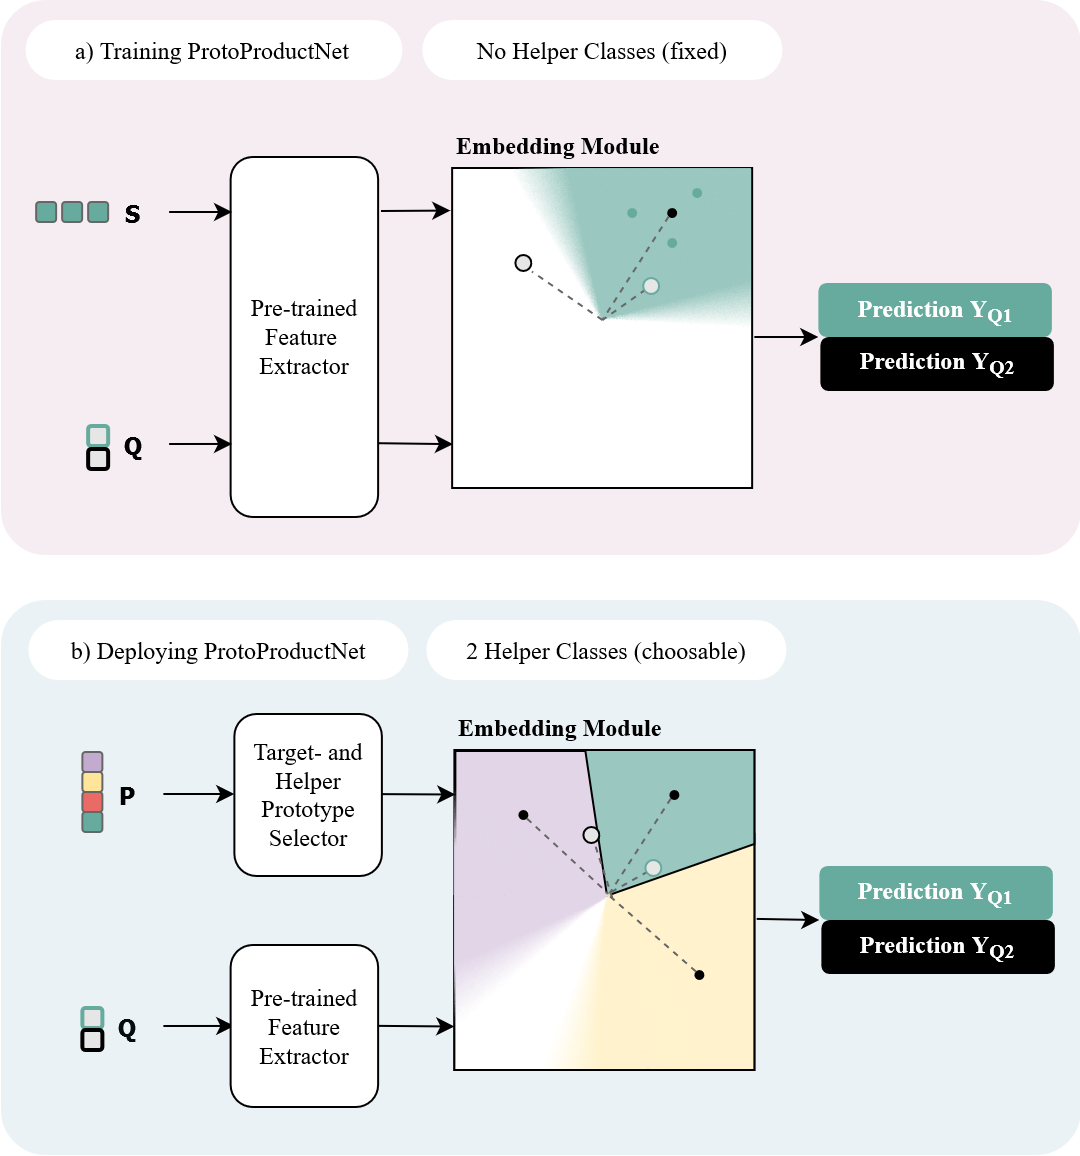
\includegraphics[width=0.95\linewidth]{rss_protoproductnet.png}
  % \end{center}
  % \caption{An overview of the architecture of ProtoProductNet during a) training; and b) deployment. Helper prototypes help distinguish close classes during inference.}
  % \label{fig:protoproductnet_overview}
% \end{figure}

